% ===========================================================================
% §3 — Manuel d'utilisation de l'application Web
% ===========================================================================
\section{Guide d'utilisation de l'application}
\label{sec:manuel}

L'application est accessible à l'adresse \appurl. Elle fonctionne dans tout
navigateur moderne, sur ordinateur comme sur téléphone ; l'interface est
bilingue (français/anglais) et offre un mode clair et un mode sombre. Le
calcul s'exécute \emph{entièrement dans le navigateur} : aucune donnée saisie
n'est transmise à un serveur, sauf si l'utilisateur enregistre explicitement
un scénario dans son compte.

\begin{figure}[t]
  \centering
  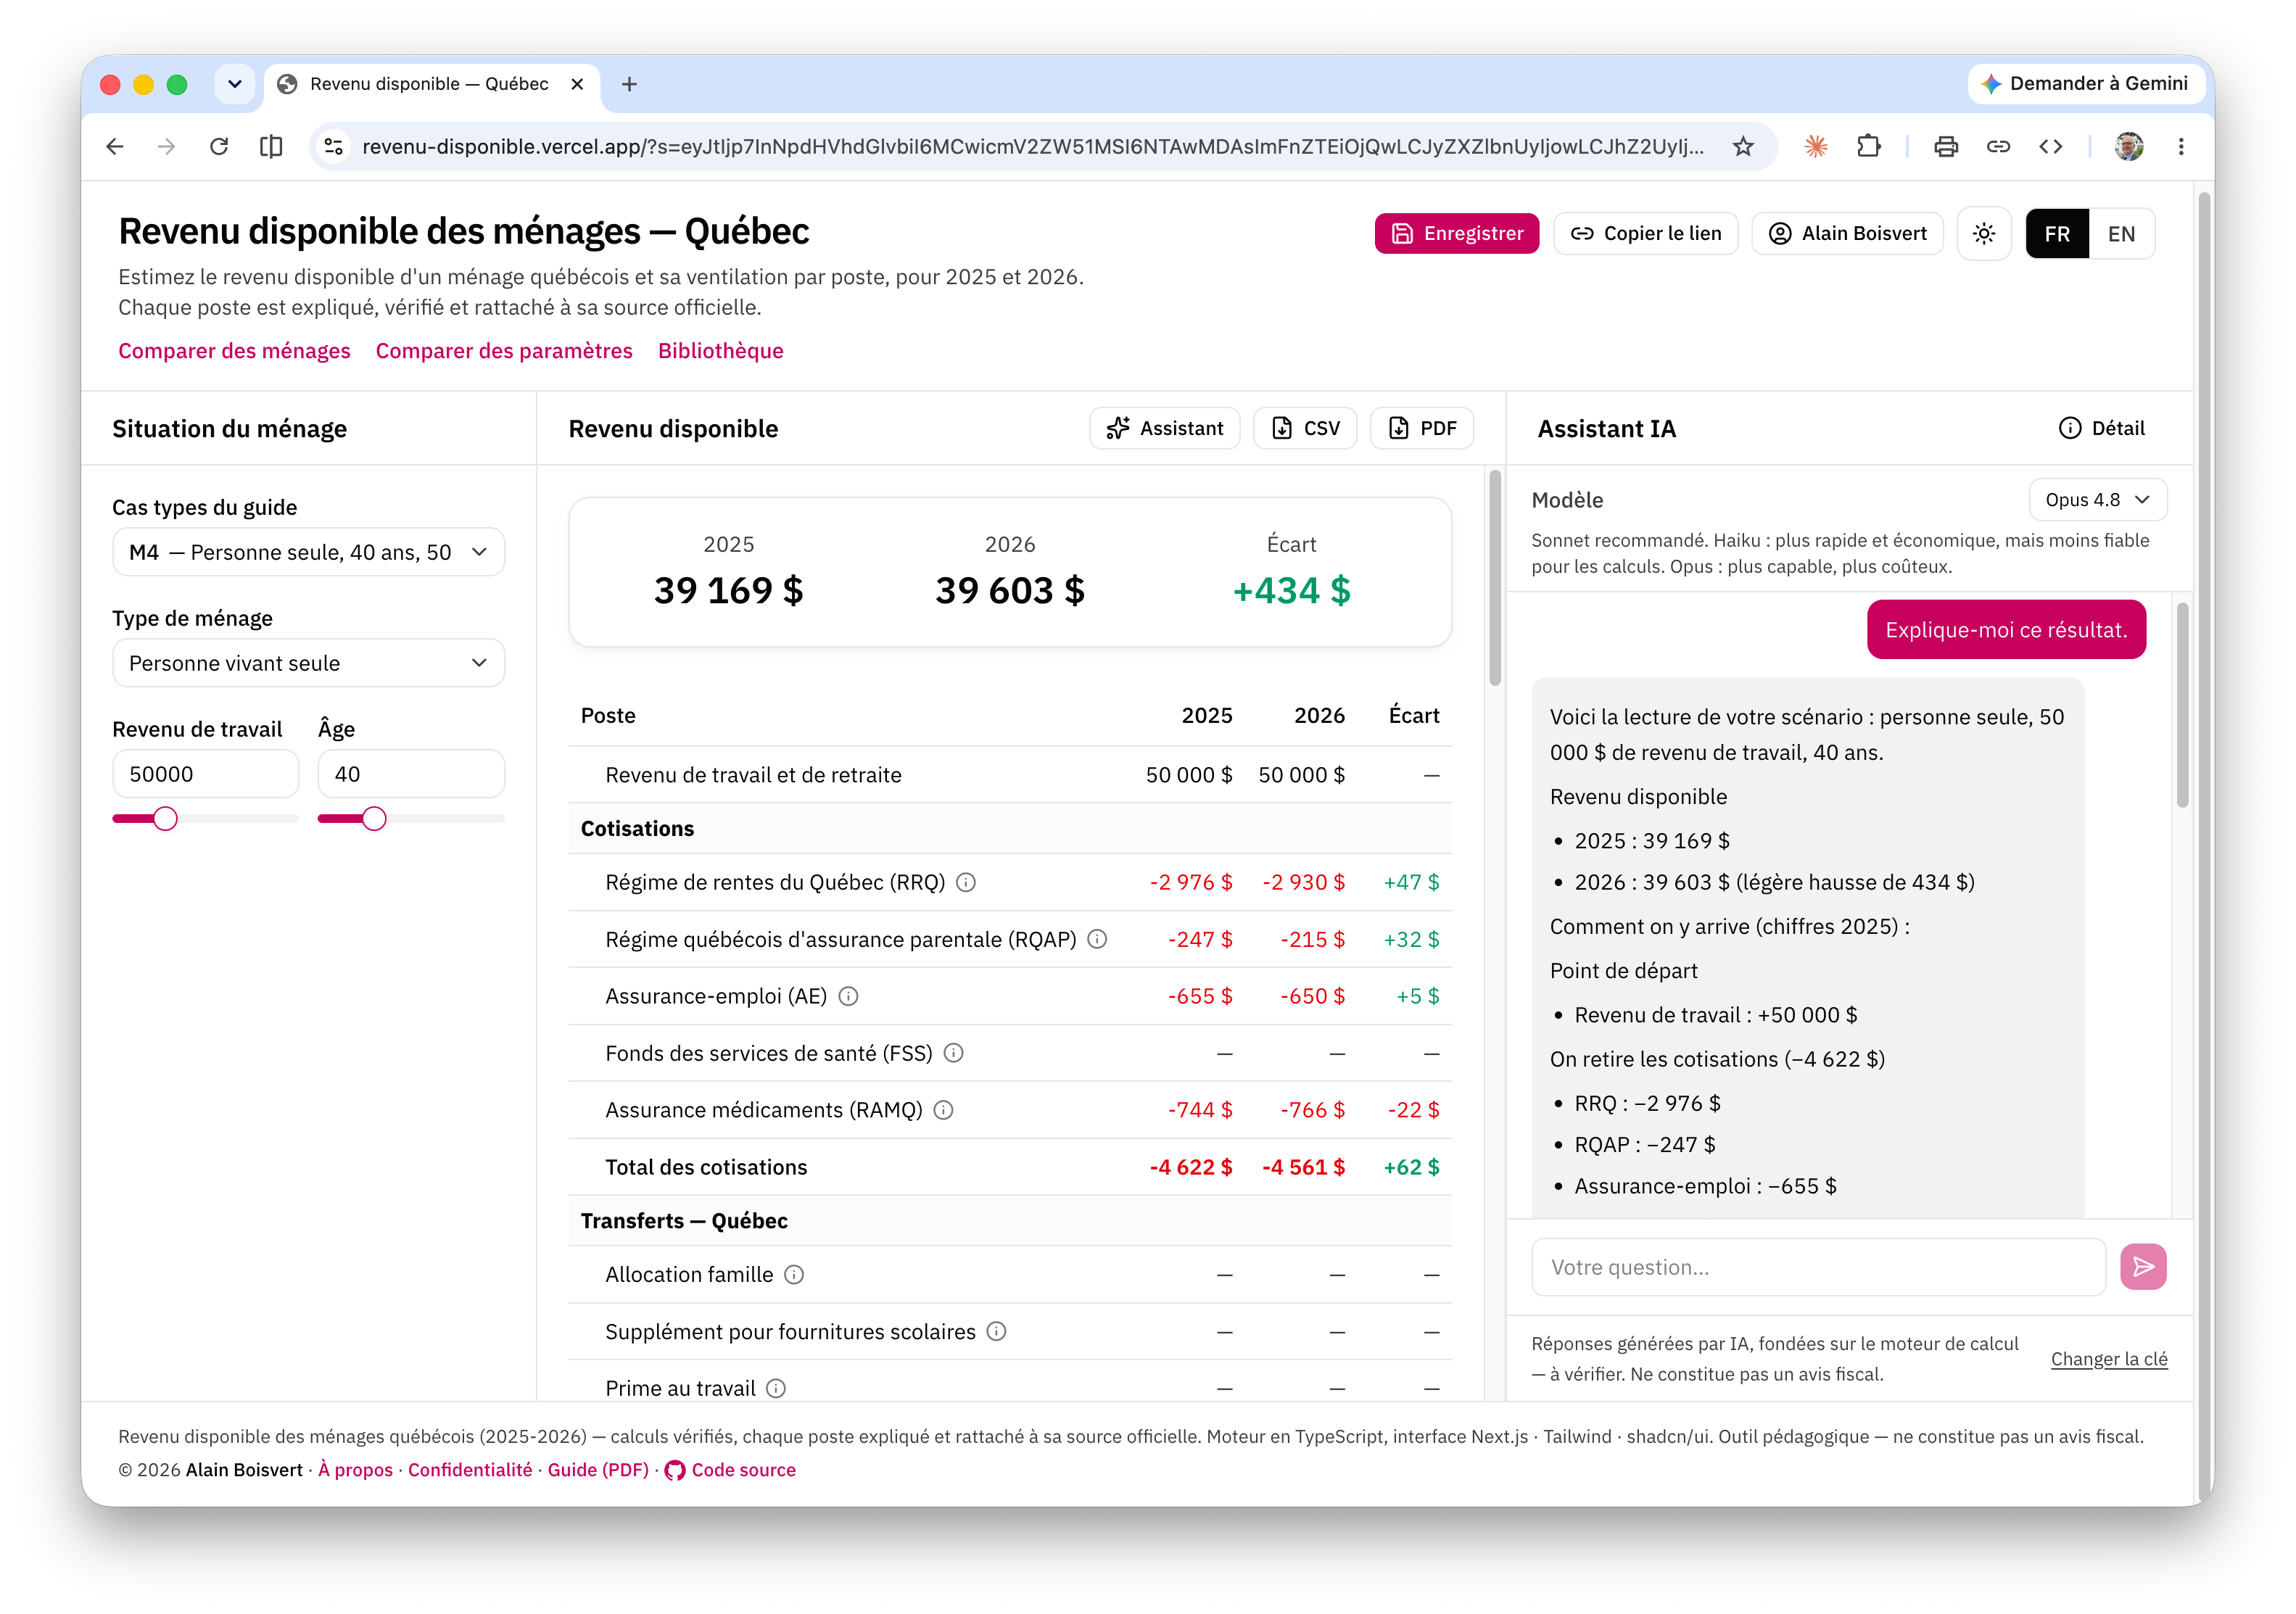
\includegraphics[width=\linewidth]{../calculateur_fr.png}
  \caption{La page principale du calculateur (interface française). De
  gauche à droite : la situation du ménage (ici, une personne vivant seule,
  \D{50000} de revenu de travail, 40~ans), le revenu disponible 2025 et
  2026 avec sa ventilation poste par poste, et le volet droit --- ici
  l'assistant d'intelligence artificielle, avec son sélecteur de modèle,
  qui explique le résultat affiché.}
  \label{fig:calculateur}
\end{figure}

\subsection{La page principale : le calculateur}

La page d'accueil est un espace de travail en trois volets redimensionnables
(figure~\ref{fig:calculateur}).

\begin{description}
  \item[Volet gauche --- la situation du ménage.] On y choisit la situation
  (tableau~\ref{tab:situations}), puis le revenu et l'âge de chaque adulte
  (champ numérique ou glissière), et le cas échéant les enfants : âge, frais
  de garde annuels et type de service (subventionné ou non).

  \item[Volet central --- les résultats.] Un bloc-résumé affiche le revenu
  disponible 2025, celui de 2026 et leur écart. Suit le tableau détaillé :
  chaque poste y apparaît sur sa ligne (cotisations, transferts québécois,
  impôt du Québec, transferts fédéraux, impôt fédéral), avec sous-totaux par
  bloc et écart 2025--2026 par ligne. L'icône~\og i \fg{} de chaque ligne
  ouvre le détail du poste dans le volet droit. Suit la carte des
  \textbf{seuils d'imposition et de contribution nette} : la position nette
  du ménage (transferts reçus moins impôts payés) et, sur une ligne de
  revenu, les seuils où il paie son premier dollar d'impôt (Québec,
  fédéral) et où il devient contributeur net
  (section~\ref{sec:seuils}). Plus bas, le
  \textbf{graphique du taux effectif marginal d'imposition} (TEMI) montre,
  pour chaque niveau de revenu de travail de 0 à \D{100000}, la part d'un
  dollar supplémentaire qui n'atteint pas le revenu disponible, décomposée
  par catégorie (cotisations, impôts, transferts récupérés), avec en
  pointillé le taux du \emph{barème d'imposition seul} ; les zones où le
  TEMI dépasse \pc{60} --- les \og trappes \fg{} --- y sont marquées en
  rouge (marquage foncé au-delà de \pc{100}), et un tableau donne la
  décomposition exacte au revenu actuel du ménage. La méthode est exposée à
  la section~\ref{sec:temi}.

  \item[Volet droit --- le détail.] Pour le poste sélectionné : description,
  objectif, règle de calcul, tableau des paramètres officiels 2025/2026 et
  références, avec lien vers la source officielle. Ce volet peut aussi
  accueillir l'\textbf{assistant d'intelligence artificielle} (voir plus
  bas).
\end{description}

Boutons utiles : \textbf{Copier le lien} encode le scénario complet dans
l'adresse URL (paramètre \texttt{?s=}) --- quiconque ouvre le lien retrouve
exactement le même ménage ; \textbf{CSV} et \textbf{PDF} exportent le tableau
des résultats ; \textbf{Enregistrer} sauvegarde le scénario dans le compte de
l'utilisateur.

\subsection{Comparer deux ménages}

La page \emph{Comparer des ménages} place deux ménages côte à côte (A et B)
sur un même jeu de paramètres et l'année choisie : le tableau central affiche
les deux décompositions et l'écart poste par poste. Utile pour mesurer, par
exemple, l'effet d'un deuxième revenu, d'un enfant de plus ou du passage à la
retraite. Survoler le titre d'un scénario rappelle sa composition.

\subsection{Comparer des paramètres (simulation de budget)}

La page \emph{Comparer des paramètres} inverse l'exercice : un \emph{même}
ménage est soumis à deux jeux de paramètres (A et B). Chaque jeu part d'une
année officielle (2025 ou 2026) et peut être modifié champ par champ ---
montants, taux, seuils et même les paliers d'imposition --- via un éditeur
organisé par poste. C'est l'outil de simulation budgétaire : que gagnerait ce
ménage si le gouvernement haussait tel seuil ou abaissait tel taux ? Par
défaut, A est l'année officielle 2025 et B l'année 2026 : l'écart montre
l'effet de l'indexation et des changements annoncés.

\subsection{La bibliothèque}

La page \emph{Bibliothèque} (connexion requise) conserve des \emph{ménages
types} et des \emph{jeux de paramètres} réutilisables dans les pages de
comparaison. Les jeux enregistrés ne stockent que les écarts par rapport aux
paramètres officiels.

\subsection{Comptes et sauvegarde}

La création de compte (courriel et mot de passe, ou compte Google) permet
d'enregistrer des scénarios et de les rouvrir plus tard. Un scénario
enregistré n'est rien d'autre que le code de partage de l'URL : aucune
donnée personnelle n'y figure au-delà de la composition fictive du ménage.

\subsection{L'assistant d'intelligence artificielle}

Le volet droit peut basculer vers un assistant conversationnel (Claude,
d'Anthropic) qui explique les résultats : pourquoi tel crédit diminue, ce qui
change entre 2025 et 2026, que se passerait-il avec \D{5000} de plus, etc.
Deux garde-fous méritent mention :

\begin{itemize}
  \item \textbf{clé personnelle} : l'assistant requiert la clé API Anthropic
        de l'utilisateur (\emph{bring your own key}), conservée localement
        dans le navigateur et jamais stockée côté serveur ; le modèle
        utilisé est sélectionnable (Haiku~4.5, Sonnet~4.6 ou Opus~4.8) ;
  \item \textbf{ancrage sur le moteur} : la ventilation exacte calculée par
        le moteur est injectée dans le contexte du modèle avec interdiction
        de recalculer --- l'assistant recopie les chiffres du moteur et
        n'invente pas les siens. Pour les questions \og et si\ldots{} ? \fg{},
        une route serveur réexécute le moteur et fournit le résultat exact à
        l'assistant.
\end{itemize}
